\chapter{Physicomimetics Desynchronization Algorithm for Single-hop Networks}
\label{chap:algo}

\section{Introduction}
\label{sec:intro-dwarf}
As we mentioned in the previous chapter, physicomimetics algorithms have been widely used for the robotic pattern formation that can be abstracted as desynchronization in the spatial domain.
One of such algorithms is that of \cite{4141997}. In their work, robots are in an artificial force field. Robots with the same type repel each other to form themselves into a circular shape. 

Inspired by their work, in this chapter, we present a novel physicomimetics desynchronization algorithm called \textit{DWARF} (Desynchronization With an ARtificial Force field) for single-hop wireless sensor networks.
Each neighboring node has artificial forces to repel other nodes to perform tasks at different time phases. Nodes with closer time phases have stronger forces to repel each other in the time domain. Each node adjusts its time phase proportionally to its received forces. Once the received forces are balanced, nodes are desynchronized

DWARF has the following key contributions:
\begin{itemize}
\item DWARF is a distributed desynchronization algorithm using time phases of all neighbors to achieve the desyncrhony state. 
\item DWARF uses only local information but achieves a global state.
\item DWARF does not require time synchronization, does not assume already slotted time, and does not incur any control message overhead.
\item DWARF is simple due to low complexity in terms of computation and memory. Therefore, it is suitable for resource-constraint networks, such as wireless sensor networks. Additionally, message complexity is low because the algorithm relies on the timing of the message, not information inside the message.
\item We have implemented and evaluated DWARF on TOSSIM, a simulator for wireless sensor networks. Our results indicate that DWARF scales well with network size and outperforms DESYNC significantly by achieving 10 - 63\% reduction in desynchronization error.
\end{itemize}
Therefore, we believe that DWARF can be a primer for various applications and can be extended for multi-hop networks which will be later described in Chapter \ref{chap:multihop}.

In the next section, we present the concept of an artificial force field which is the crucial concept of our desynchronization algorithm.

\section{Artificial Force Field}
\label{sec:forcefield}
An artificial force field is an analogy to the circle of a time period.
Nodes are in the same force field if they can communicate with each other. 

If node $i$ and node $j$ are on the same force field, they have repelling forces to push one another away. 
A closer pair of nodes has a higher magnitude of force than a farther pair does.
The time interval between two nodes is derived from the phase difference between them.
If two nodes have a small phase difference, they have a high magnitude of force and vice versa.
In other words, a repelling force is an inverse of a phase difference between two nodes:
\begin{equation}
f_{i,j} = - \frac{1}{\Delta \phi_{i,j} / T} , \Delta \phi_{i,j} \in (-\frac{T}{2}, \frac{T}{2}),
\label{eq:force}
\end{equation}
where $f_{i,j}$ is the repelling force from node $j$ to node $i$ on a time period $T$ and $\Delta \phi_{i,j}$ is the phase difference between node $i$ and $j$.
We note that $\Delta \phi_{i,j}$ is not equal to 0 because if two nodes fire at the same time, their firings collide and two nodes do not record other's firing. Additionally, at $T/2$ or $-T/2$, a node does not repel an opposite node because they are balanced.

A repelling force can be positive (clockwise repelling) or negative (counterclockwise repelling).
A positive force is created by a node on the left half of the circle relative to the considered node whereas a negative force is created by a node on the right half.
Figure \ref{fig:force_field} represents a field of repelling forces on node 1. 

\begin{figure}[!t]
\centering
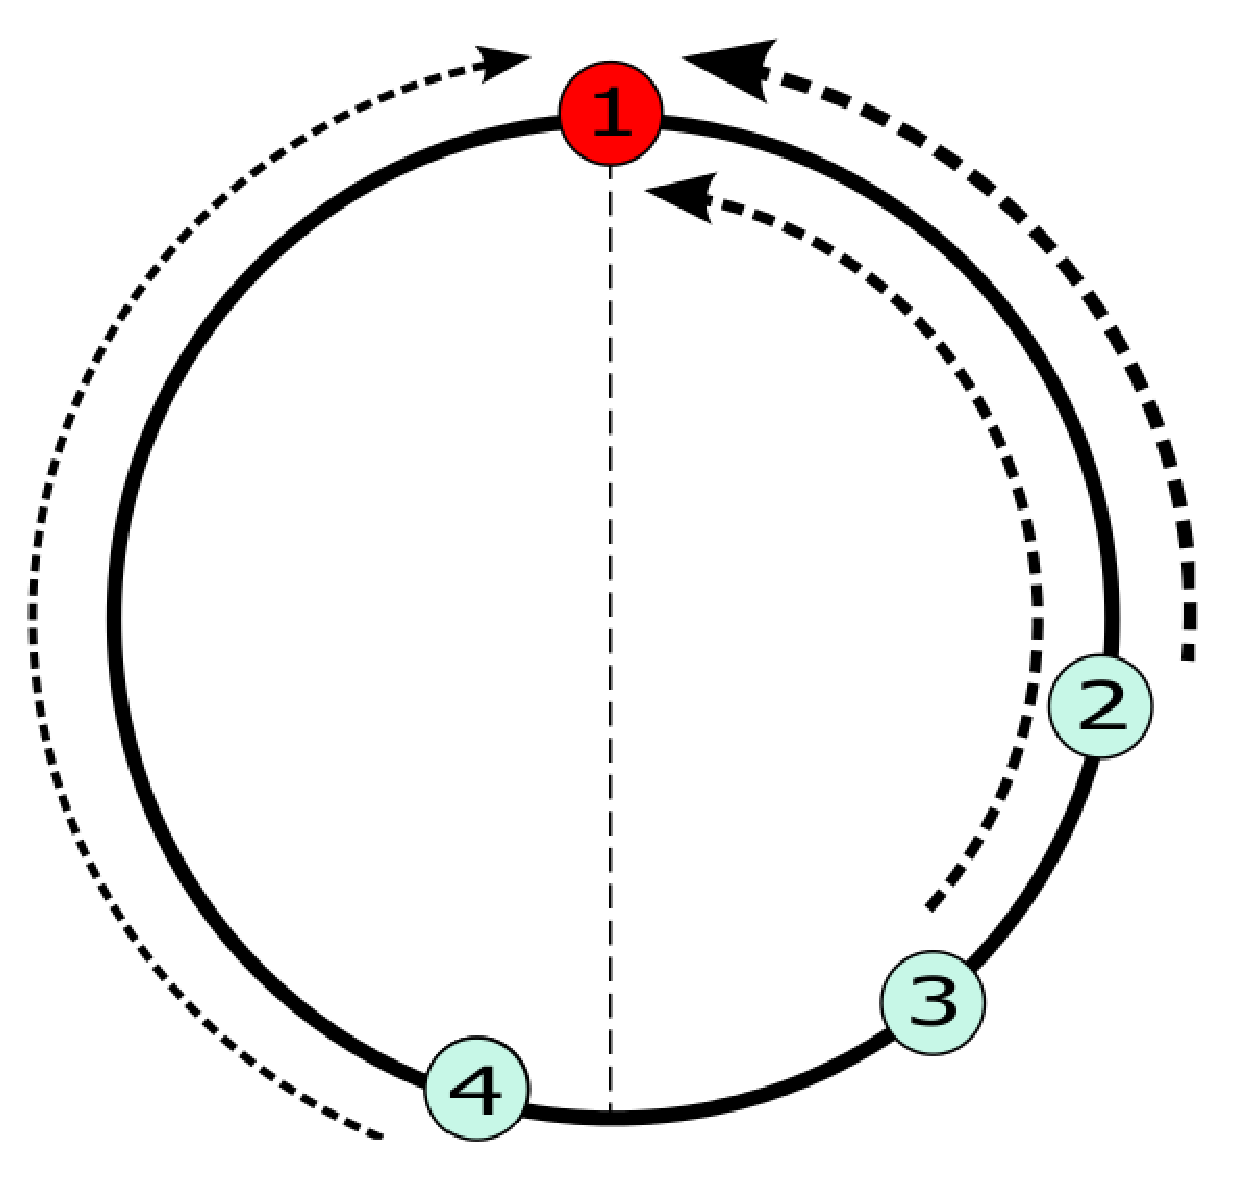
\includegraphics[width=2.2in]{figure/forcefield}
\caption{Artificial Force Field. Arrow lines represent repelling forces from node 2, 3, and 4 to node 1. A shorter and thicker line is a stronger force. A force from node 4 is a positive force and two forces from node 2 and 3 are negative forces.}
\label{fig:force_field}
\end{figure}

Each node in the force field moves to a new time position or phase proportional to the total received force.
Given $n$ nodes in a force field, the total force on a node $i$ is the following:
\begin{equation}
\mathcal{F}_i = \sum_{\substack{j=1\\ j \neq i}}^{n}{f_{i,j}}.
\label{eq:fsum}
\end{equation}
Eventually, nodes reach an equilibrium state whereby the total force of the system is close to zero and each pair of phase neighboring nodes has the same time interval.
This equilibrium state also indicates the perfect desynchrony state because all nodes are equally spaced on the time circle.

\section{Algorithm}
\label{sec:algo}
We assume that, initially, nodes are not desynchronized. 
Each node sets a timer to fire in $T$ time unit.
After setting the timer, each node listens to all neighbors until its timer expires.

When receiving a firing message from its neighbor, the (positive or negative) repelling force from that neighbor is calculated based on the phase difference.
When the timer expires, a node broadcasts a firing message to neighbors. 
Then, the node calculates a new time phase to move on the circle based on the summation of forces from all neighbors and sets a new timer according to the new time phase.

Reasonably, one may wonder how far a node should move or adjust its phase.
In our work, given the total received force $\mathcal{F}_i$, the node $i$ adjusts to a new time phase $\phi_i^{'}$,
\begin{equation}
\phi_i^{'} = (\phi_i + K\mathcal{F}_i) \mod T,
\label{eq:newphase}
\end{equation} 
where $\phi_i$ is the current phase of the node $i$.

Undoubtedly, the proper value of the coefficient $K$ leads to the proper new phase.
The value of $K$ is similar to a step size which is used in artificial intelligence techniques. 
Therefore, if the value of $K$ is too small, the system takes much time to converge. 
On the other hand, if the value of $K$ is too large, the system may overshoot the optimal value and does not converge. 
We observe that, given the same time period, fewer nodes in the system result in bigger phase difference between two phase neighbors. To be desynchronized, nodes in sparse networks must make a bigger adjustment to their time phases than nodes in dense networks must.
Therefore, the same total received force should have a bigger impact on a node in sparse networks than on a node in dense networks. 
To reflect this observation, the coefficient $K$ is inversely proportional to a power of the number of nodes $n$,
\begin{equation}
K = c_1 \times n^{-c_2}, \text{ where } c_1, c_2 \geq 0.
\end{equation}

Therefore, we have conducted an experiment to find the proper value of $c_1$ and $c_2$. 

We set a time period $T$ to 1000 and vary the number of nodes.
In the specific number of nodes, we first simulate to see the trend of the value $K$ that leads to small errors. 
Then, we select a range of good $K$ values. 
After that, we simulate 100 times to obtain the average desynchronization error for each $K$ value. 
In each simulation, we randomly set an initial phase of each node between 0 and $T$ (period value). 
Finally, we select the $K$ value that results in the lowest error. 
After getting the proper $K$ value for each number of nodes, we plot the relation between $K$ and the number of nodes (Figure \ref{fig:relation_k_n}) and use a mathematical tool to calculate the power regression. The obtained relation function between $K$ and $n$ (the trendline in Figure \ref{fig:relation_k_n}) consists of $c_1$ and $c_2$  values as follows:
\begin{equation}
K = 38.597 \times n^{-1.874}.  \nonumber
\end{equation}
However, this $K$ value is derived by setting $T$ equal to 1000. 
Therefore, for arbitrary $T$, 
\begin{equation}
K = 38.597 \times n^{-1.874} \times \frac{T}{1000}.
\end{equation}
\begin{proof}
From Equation \ref{eq:fsum} and \ref{eq:newphase}, the phase of node $j$ is adjusted by $K\mathcal{F}_{j} = K\sum_{i \neq j}^n f_{i,j} = \sum_{i \neq j}^n K f_{i,j}$.
Therefore, we can analyze the value of $K$ from only single force $f_{i,j}$.

\begin{figure}[!t]
\centering
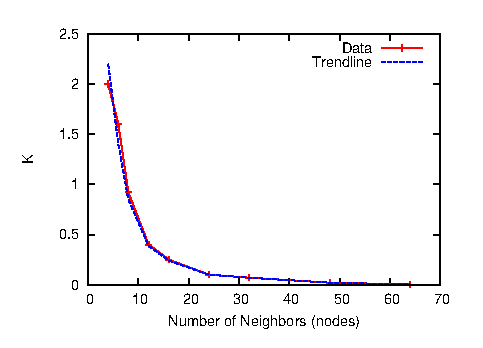
\includegraphics[width=3.5in]{figure/k-trendline}
\caption{Relation of the coefficient $K$ with a number of nodes $n$}
\label{fig:relation_k_n}
\end{figure}

For a time circle of a period $T_{p}$, let $\theta_{p}$ be an angle between two nodes on the circle and $\Theta_{p}$ be an angle between the new adjusted phase and the old phase based on a single force where $\theta_{p}, \Theta_{p} \in (0, 2\pi)$. %and let its value equal to a normalized phase difference $\Delta \phi_{i,j} / T_{p}$ and $\theta^{'}_{p}$ be a new angle after adjustment.
Hence,
\begin{equation}
\frac{\theta_{p}}{2\pi}  = \frac{\Delta \phi_{i,j}}{T_p},
\label{eq:theta}
\end{equation}
and 
\begin{equation}
\frac{\Theta_{p}}{2\pi}  = \frac{Kf_{i,j}}{T_p}.
\label{eq:Theta}
\end{equation}
If $\theta_1$ of $T_1$ equals to $\theta_2$ of $T_2$, both of them should be adjusted with the same angle amount $\Theta_{1}$ = $\Theta_{2}$. 
Thus, from Equation \ref{eq:Theta},
\begin{alignat}{2}
\Theta_1 =&  \text{ } \Theta_2 \nonumber \\
\frac{K_{1} f_{i,j(1)}}{T_1} =& \text{ } \frac{K_{2} f_{i,j(2)}}{T_2}.  \nonumber
\end{alignat}
From Equation \ref{eq:force} and \ref{eq:theta}, $f_{i,j} = \frac{1}{\Delta \phi_{i,j} / T_{p}} = \frac{2\pi}{\theta_{p}}$, consequently,
\begin{alignat}{2}
\frac{K_{1}2\pi}{T_1\theta_1} =& \text{ } \frac{K_{2}2\pi}{T_2\theta_2}  \nonumber \\
\frac{K_{1}}{T_1} =& \text{ } \frac{K_{2}}{T_2}  \nonumber \\
K_2=& \text{ } K_{1} \frac{T_2}{T_1}.  \label{eq:k-k}
\end{alignat}
At $T = 1000$, we get $K = 38.597 \times n^{-1.874}$.
Therefore, from Equation \ref{eq:k-k}, for arbitrary $T$,
\begin{equation}
K = 38.597 \times n^{-1.874} \times \frac{T}{1000}. \nonumber
\end{equation}
\end{proof}


All nodes in the artificial force field (in the period circle) iteratively run the same algorithm until the force is balanced (\textit{i.e.}, all nodes are in the desynchrony state).
The pseudo-code of this algorithm is shown in Figure \ref{fig:pseudocodedwarf}.

\begin{figure}[!t]
\begin{algorithmic}[1]
	\STATE \textbf{Initialization}  
  	\STATE $T = TimePeriod$ \COMMENT{Configurable Time Period}
  	\STATE $n = 1$ \COMMENT{Number of receiving messages including itself}
  	\STATE $\mathcal{F} = 0$ \COMMENT{Force Summation}
  	\STATE $lastFiringTime = localTime$
  	\STATE $currentPhase = localTime$ modulo $T$
  	\STATE Set a firing timer to be $T$ unit time
  	\newline
  	
  	\STATE \textbf{Upon timer firing}
    \STATE Broadcast a firing message to neighbors
    \STATE $lastFiringTime = localTime$
  	\STATE $currentPhase= localTime$ modulo $T$
    \STATE $K = 38.597 \times n^{-1.874} \times \frac{T}{1000}$
    \STATE $newPhase = currentPhase + (K \times \mathcal{F})$
    \IF{$newPhase < 0$}
    	\STATE $newPhase = T + newPhase$
	\ENDIF
    \STATE Set a firing timer to be fired at ($newPhase$ modulo $T$)
   	\STATE $\mathcal{F} = 0$
   	\STATE $n = 1$
 	\newline
 	   
    \STATE \textbf{Upon receiving a firing message}
    \STATE $n = n + 1$
    \STATE $phaseDiff = localTime - lastFiringTime$
    \IF{$phaseDiff == 0.5T$} 
    	\STATE $\mathcal{F} = \mathcal{F} + 0$ \COMMENT{Balanced force}
    \ELSIF{$phaseDiff < 0.5T$} 
    	\STATE $\mathcal{F} = \mathcal{F} + |\frac{1}{phaseDiff / T}|$  \COMMENT{Positive force}
   	\ELSE 
   		\STATE $\mathcal{F} = \mathcal{F} - |\frac{1}{(T - phaseDiff) / T}|$ \COMMENT{Negative force}
    \ENDIF
\end{algorithmic}
\caption{Pseudocode of DWARF algorithm}
\label{fig:pseudocodedwarf}
\end{figure}

\section{Evaluation}
In this section, we evaluate the performance of our proposed algorithm and compare with DESYNC (\cite{4379660}) because DESYNC and our algorithm share the same goal and requirements. Particularly, they do not require time synchronization, do not assume already slotted time, do not need to look into the packet content, and do not incur control packets but still achieve equivalent time spaces. Other protocols (\textit{e.g.}, M-DESYNC (\cite{4274893}), Lightweight desynchronization (\cite{5062165})) assume different requirements. Therefore, we only discuss our differences with such protocols in Chapter \ref{chap:related}.

The performance metrics in this evaluation are desynchronization error and convergence time. The former indicates how close the current state is to the perfect desynchrony state. The latter indicates how fast the algorithm converges.

\subsection{Evaluation Environment}
We implement DWARF on TinyOS 2.1.2 (\cite{levis-tinyos-04}), an operating system for wireless sensor networks
and evaluate the protocol on TOSSIM (\cite{levis-tossim-03}), a TinyOS simulator.
We vary the one-hop network size from 4 to 96 nodes.
Each node periodically fires a message that contains only application data with no extra control overhead.
%The message does not contain any overhead. 
This zero overhead is the advantage of both DWARF and DESYNC because, to avoid collision, a node only needs to know the timing of the firing rather than the control information inside a packet. 
In our simulation, for both DWARF and DESYNC, we use a 2-byte node ID and a 2-byte counter as the data. However, we do use the regular 11-byte CC2420 header for TOSSIM.
Therefore, we do not measure the overhead in our evaluation.
We set the time period to 1,000 milliseconds and compare our result with that of DESYNC.
Initially, the phase of each node is random in a range of 0 to 1,000.

\subsection{Varying Step Size in DESYNC}
\label{sec:varystepsize}
In \cite{4379660}, they choose the step size of DESYNC to be 0.95. In this section, we begin by varying the step size of DESYNC to confirm that the step size 0.95 is a proper and fair value for DESYNC to compare with DWARF in our investigated scenario.
Figure \ref{fig:desync-vary-small}, \ref{fig:desync-vary-medium}, and \ref{fig:desync-vary-large} show the results of varying step size from 0.10 to 0.95.
\begin{figure*}%
\centering
	\subfloat[$\alpha$ = 0.10]{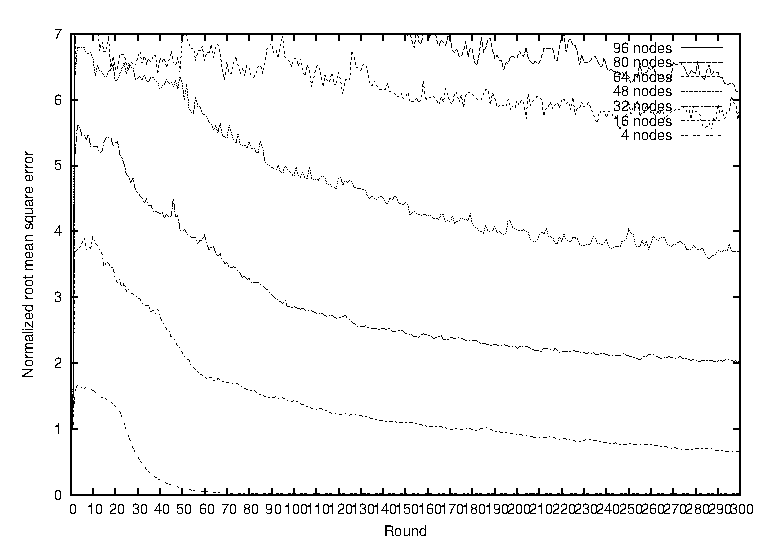
\includegraphics[width=2.5in]{figure/desync-0-10}%
	\label{fig:alpha010}}
	\subfloat[$\alpha$ = 0.15]{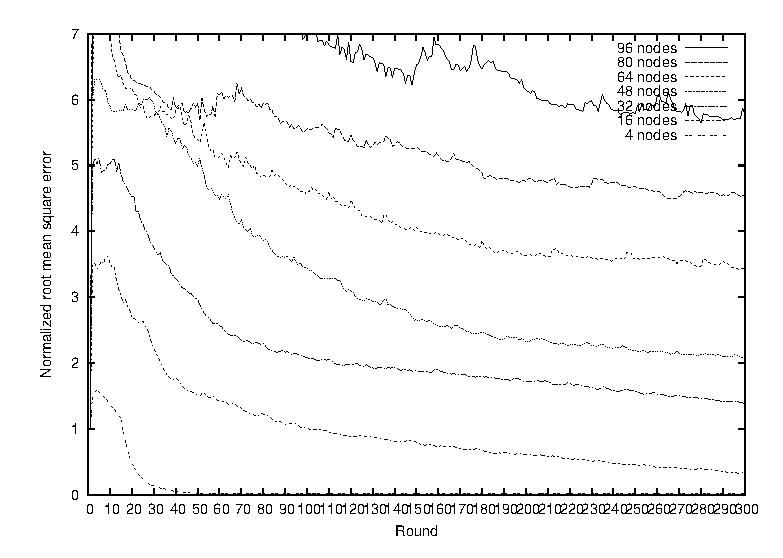
\includegraphics[width=2.5in]{figure/desync-0-15}%
	\label{fig:alpha015}}
    \hspace{8pt}%
	\subfloat[$\alpha$ = 0.20]{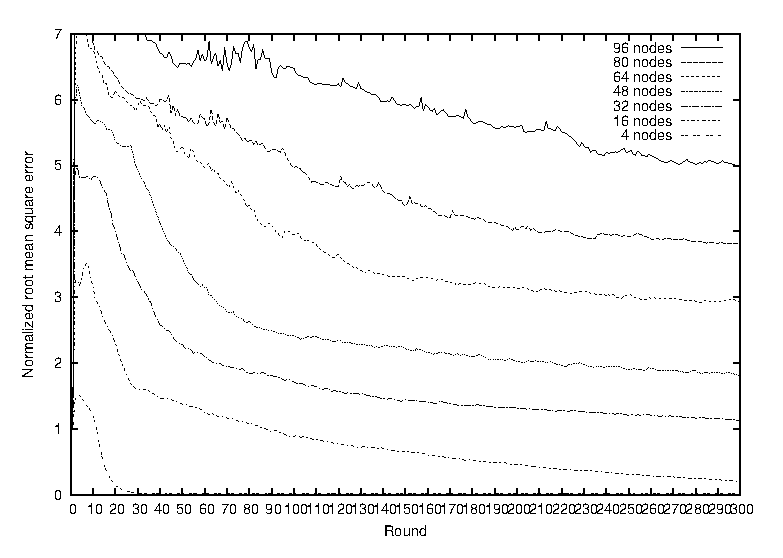
\includegraphics[width=2.5in]{figure/desync-0-20}%
	\label{fig:alpha020}}
	\subfloat[$\alpha$ = 0.25]{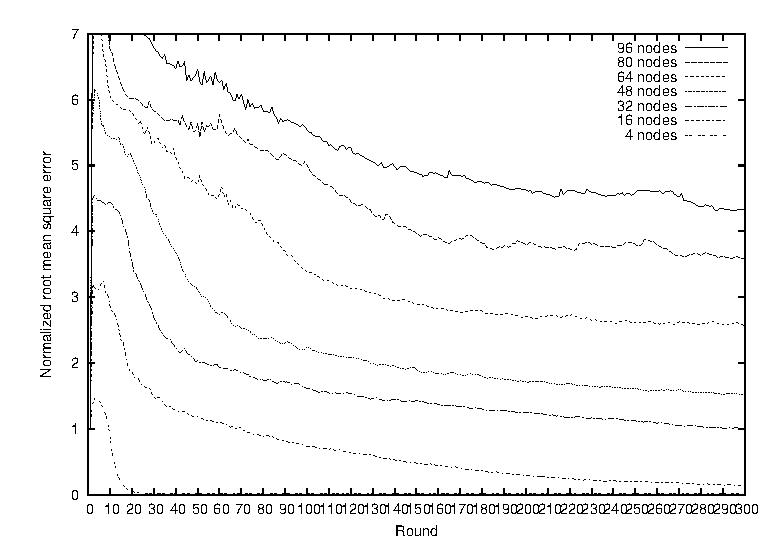
\includegraphics[width=2.5in]{figure/desync-0-25}%
	\label{fig:alpha025}}
    \hspace{8pt}%
	\subfloat[$\alpha$ = 0.30]{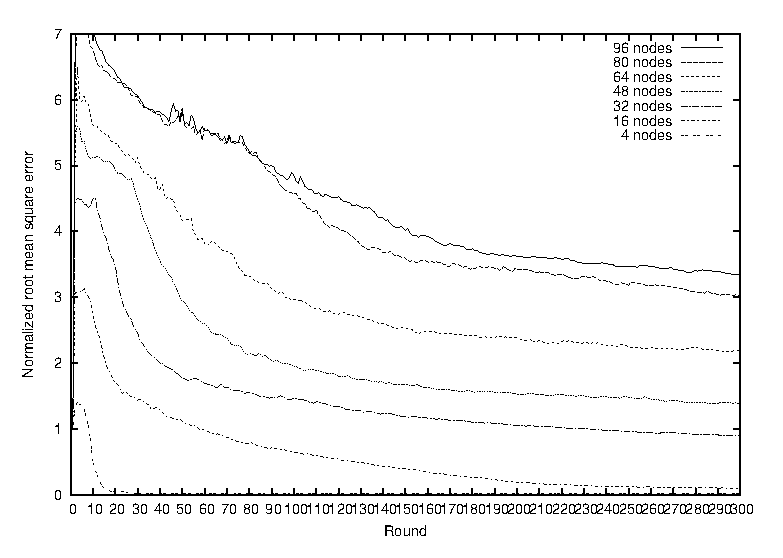
\includegraphics[width=2.5in]{figure/desync-0-30}%
	\label{fig:alpha030}}
	\subfloat[$\alpha$ = 0.35]{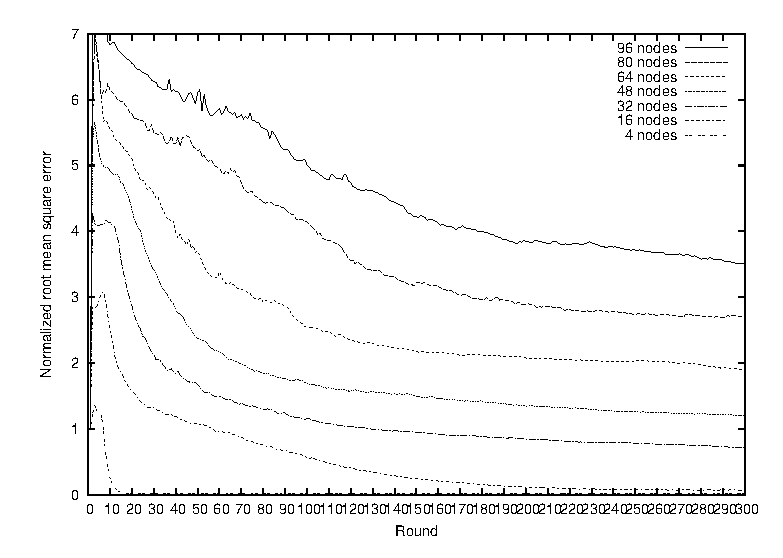
\includegraphics[width=2.5in]{figure/desync-0-35}%
	\label{fig:alpha035}}
\caption{DESYNC: Varying step size from 0.10 to 0.35}%
\label{fig:desync-vary-small}%
\lofcont
\end{figure*}

\begin{figure*}%
\centering
	\subfloat[$\alpha$ = 0.40]{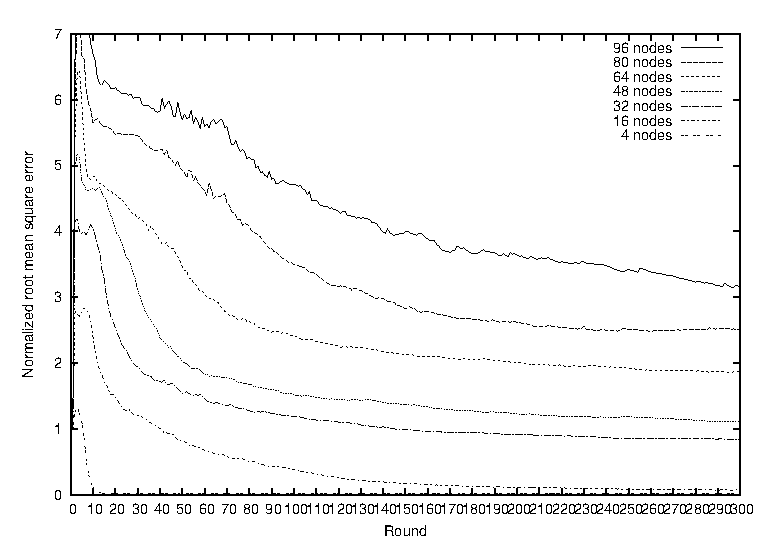
\includegraphics[width=2.5in]{figure/desync-0-40}%
	\label{fig:alpha040}}
	\subfloat[$\alpha$ = 0.45]{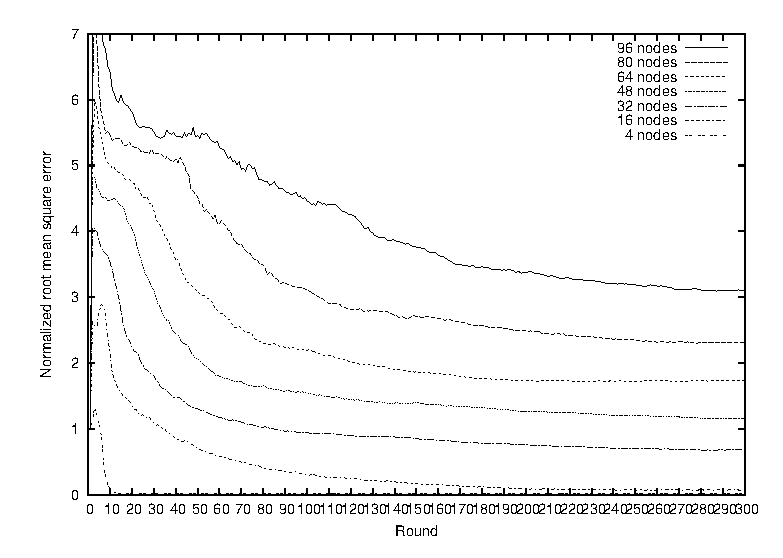
\includegraphics[width=2.5in]{figure/desync-0-45}%
	\label{fig:alpha045}}
    \hspace{8pt}%
	\subfloat[$\alpha$ = 0.50]{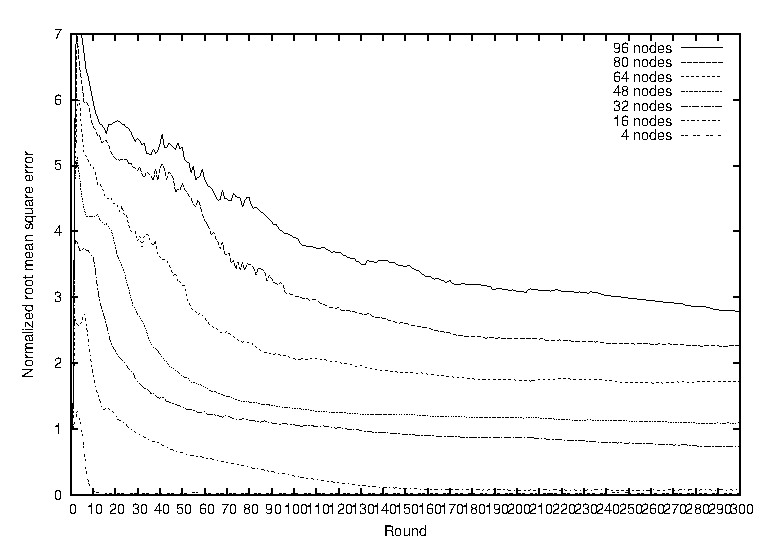
\includegraphics[width=2.5in]{figure/desync-0-50}%
	\label{fig:alpha050}}
	\subfloat[$\alpha$ = 0.55]{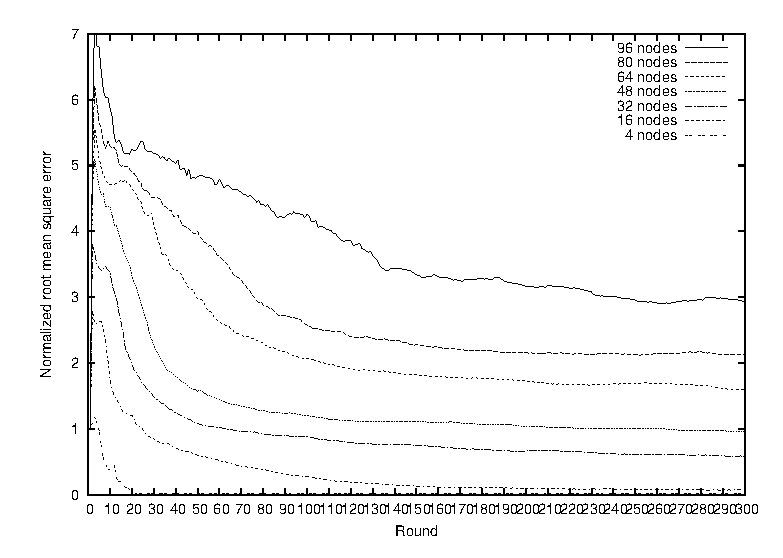
\includegraphics[width=2.5in]{figure/desync-0-55}%
	\label{fig:alpha055}}
    \hspace{8pt}%
	\subfloat[$\alpha$ = 0.60]{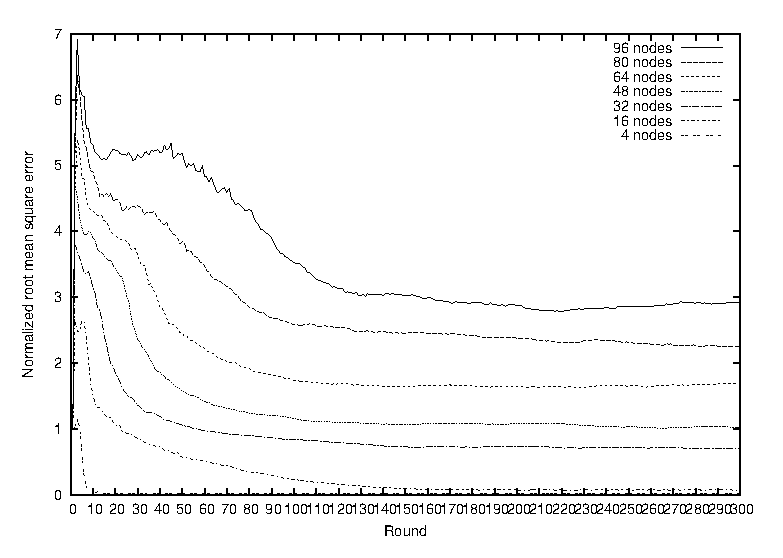
\includegraphics[width=2.5in]{figure/desync-0-60}%
	\label{fig:alpha060}}
	\subfloat[$\alpha$ = 0.65]{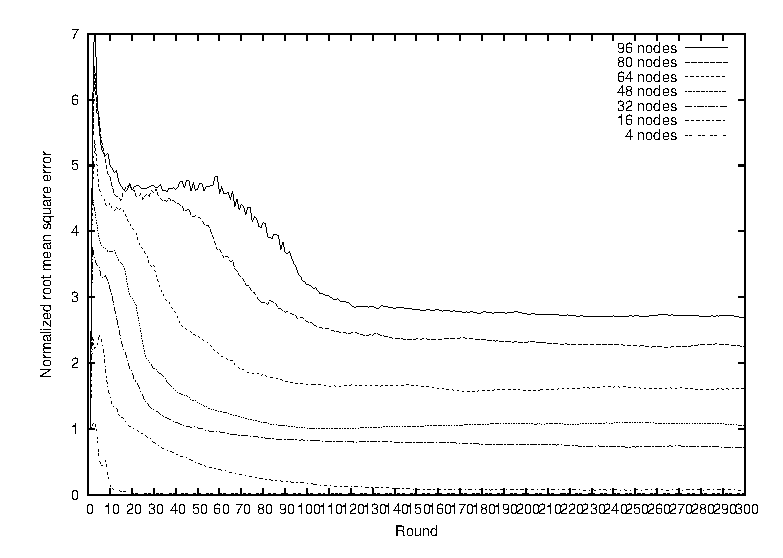
\includegraphics[width=2.5in]{figure/desync-0-65}%
	\label{fig:alpha065}}
\caption{DESYNC: Varying step size from 0.40 to 0.65}%
\label{fig:desync-vary-medium}%
\lofcont
\end{figure*}

\begin{figure*}%
\centering
	\subfloat[$\alpha$ = 0.70]{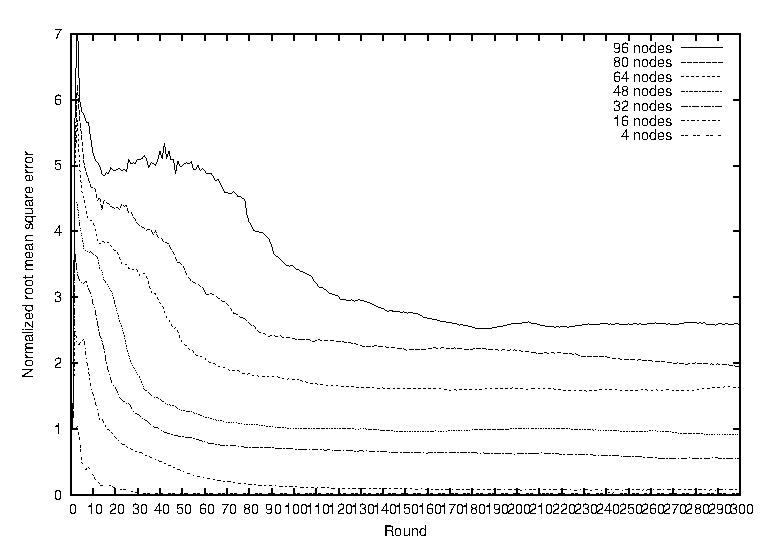
\includegraphics[width=2.5in]{figure/desync-0-70}%
	\label{fig:alpha070}}
	\subfloat[$\alpha$ = 0.75]{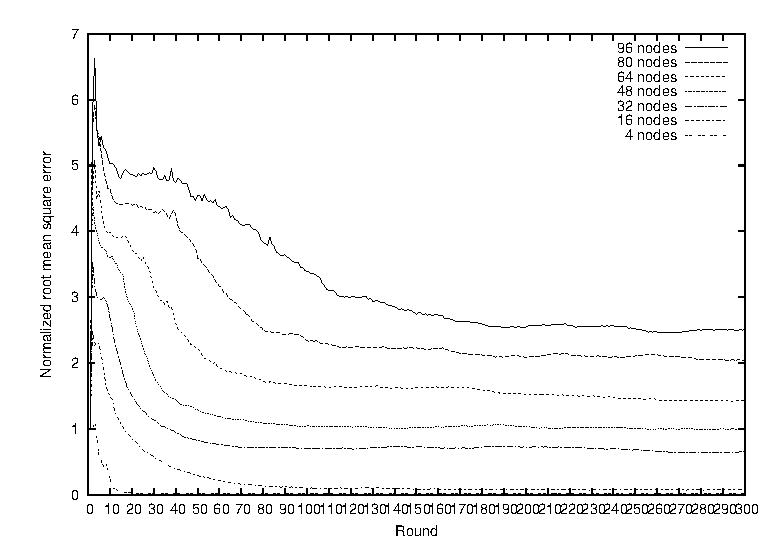
\includegraphics[width=2.5in]{figure/desync-0-75}%
	\label{fig:alpha075}}
    \hspace{8pt}%
	\subfloat[$\alpha$ = 0.80]{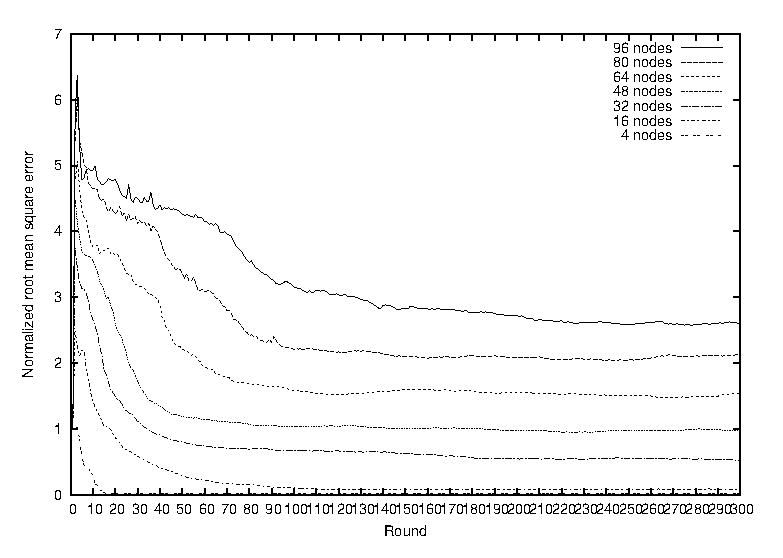
\includegraphics[width=2.5in]{figure/desync-0-80}%
	\label{fig:alpha080}}
	\subfloat[$\alpha$ = 0.85]{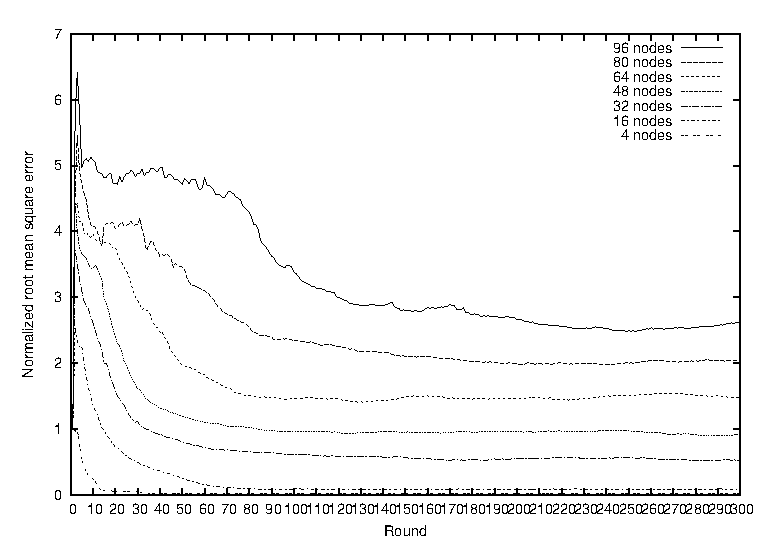
\includegraphics[width=2.5in]{figure/desync-0-85}%
	\label{fig:alpha085}}
    \hspace{8pt}%
	\subfloat[$\alpha$ = 0.90]{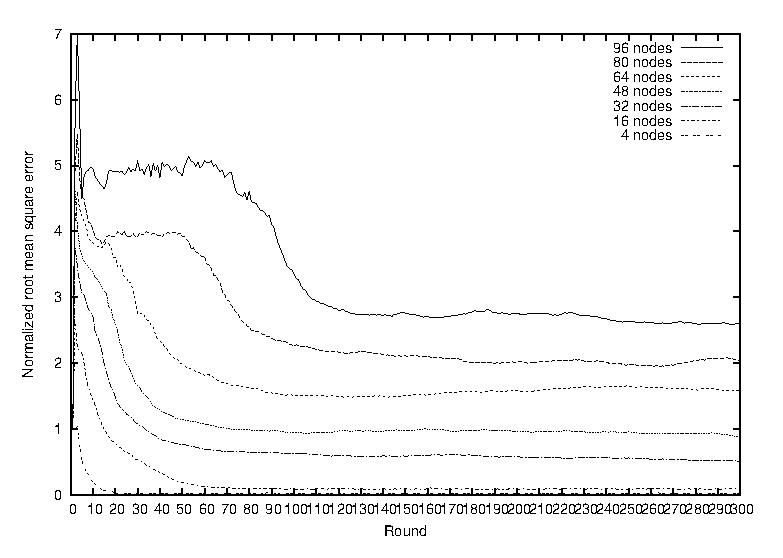
\includegraphics[width=2.5in]{figure/desync-0-90}%
	\label{fig:alpha090}}
	\subfloat[$\alpha$ = 0.95]{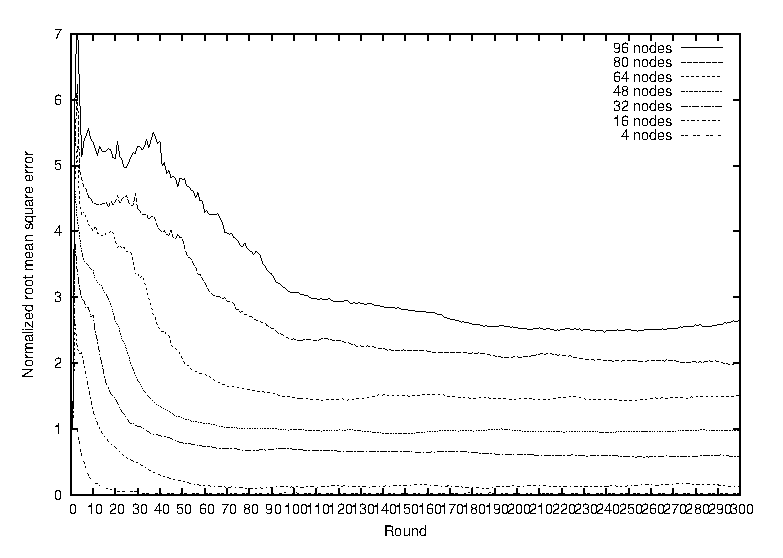
\includegraphics[width=2.5in]{figure/desync-0-95}%
	\label{fig:alpha095}}
\caption{DESYNC: Varying step size from 0.70 to 0.95}%
\label{fig:desync-vary-large}%
\lofcont
\end{figure*}

The result indicates that too small step size (0.10 to 0.35) leads to slow convergence speed and high error.
Increasing step size tends to lead to lower error. Step sizes from 0.65 to 0.95 do not result in much different in term of error but the larger value tends to lead to faster convergence speed.
However, increasing step size from 0.80 to 0.95 does not significantly improve the performance. Therefore, we can use 0.95  which is the same value used in \cite{4379660} as the step size for DESYNC to compare with DWARF.

\subsection{Desynchronization Error}
\label{sec:error}
To measure the desynchronization error, we run the simulation for 300 time periods. 
In each network size, we run the simulation for 30 times.
Then, we measure the average root mean square error (RMSE). The error (ERR) is the measured phase difference minus the perfect phase difference:

\begin{equation}
ERR_i = \Delta \phi_{i,j} - T/n, \nonumber
\end{equation}
\begin{equation}
RMSE = \sqrt{\frac{\sum_{i = 1}^{n}{ERR_i^2}}{n}}, \nonumber
\end{equation}
where node $j$ is the next phase neighbor of node $i$.
$\Delta \phi_{i,j}$ is the phase difference between node $i$ and node $j$ on the time period $T$.
Given that $n$ is a total number of nodes, $T/n$ is the perfect phase difference.

%Figure \ref{fig:rmse300rounds} illustrates the result of the desynchronization error in each network size after 300 time periods.
However, a smaller absolute error in a dense network is not necessarily better than a bigger error in a sparse network because the perfect phase difference in a dense network is also smaller than that in a sparse network.
Thus, for a comparable view of each network size, we also measure a normalized root mean square error (NRMSE) that is a ratio of the root mean square error and the perfect phase difference of each network size.
% (see Figure \ref{fig:nrmse300rounds}).
Figure  \ref{fig:rmse300rounds} illustrate the result of absolute desynchronization error and Figure \ref{fig:nrmse300rounds} illustrates the result of the normalized desynchronization error in each network size after 300 time periods.

\begin{figure}[!t]
\centering
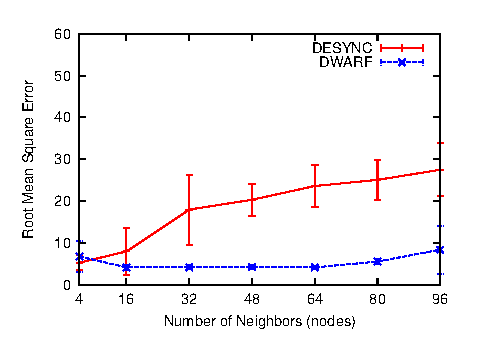
\includegraphics[width=3.0in]{figure/compare300rounds_rmse_sd}
\caption{Root mean square error after 300 time periods}
\label{fig:rmse300rounds}
\end{figure}

\begin{figure}[!t]
\centering
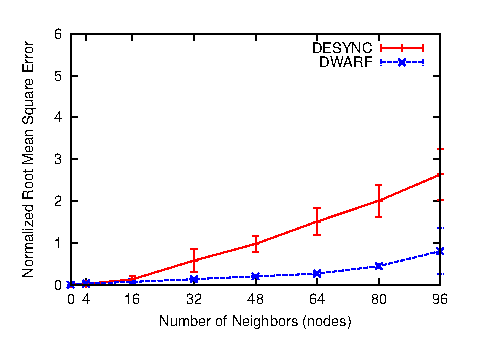
\includegraphics[width=3.0in]{figure/compare300rounds_nrmse-expected_sd}
\caption{Root mean square error normalized by perfect phase difference after 300 time periods}
\label{fig:nrmse300rounds}
\end{figure}

The result indicates that, in all network sizes (4 - 96 nodes), DWARF achieves significantly better  desynchrony states than DESYNC does.
Understandably, using information from all neighbors (as in DWARF) leads to lower errors than using information from only two phase neighbors (as in DESYNC) does. Furthermore, DESYNC's mechanism allows a phase error of a node to propagate to its phase neighbors. A part of this error will propagate back and forth between two phase neighbors as well as circulate inside the network. As a result, DESYNC's error after convergence is still quite large.
In contrast, DWARF is robust to this error propagation. Even though the error propagation may still occur, the impact is not significant. Given that DWARF uses the sum of forces from all neighbors, an error from one neighbor does not overwhelm the system.

We note that we show RMSE and NRMSE after 300 periods because, by that time, the errors of all simulation scenarios seem to be stable. The actual convergence time in most scenarios is much lower than 300 rounds (see the next section).

\subsection{Convergence Time}
\label{sec:converge}
In the desynchronization error evaluation, we only measure the performance after 300 time periods.
However, the previous result does not indicate whether the protocols have converged or not.
Neither does it indicate how fast the protocols have converged. 
Hence, we also measure the absolute root mean square error and normalized root mean square error for each time period.

In sparse networks (Figure \ref{fig:rmse-sparse} and \ref{fig:nrmse-sparse}), both protocols converge with similar small error but DWARF converges slightly faster. 
In dense networks (Figure \ref{fig:rmse-dense} and \ref{fig:nrmse-dense}) and extremely dense networks (Figure \ref{fig:rmse-extreme} and \ref{fig:nrmse-extreme}), both protocols still converge.
Even though DESYNC converges faster in such networks, it converges with a relatively high error compared to that of DWARF.
In addition, at the time when DESYNC has converged and DWARF has not converged yet, DWARF's error is already lower than DESYNC's.
Furthermore, in dense and extremely dense networks, the normalized root mean square errors of DESYNC after convergence is higher or equal to 1.
This means that the error is very large compared to the perfect phase difference.
Conversely, the normalized error of DWARF is lower than 1 even in the extremely dense networks.
Therefore, DWARF scales well with the network density whereas DESYNC does not.

In a denser network, the errors of DESYNC and DWARF are higher because the probability of message collisions increases (see the next section). 


\begin{figure*}[!t]
\centerline{
	\subfloat[Sparse]{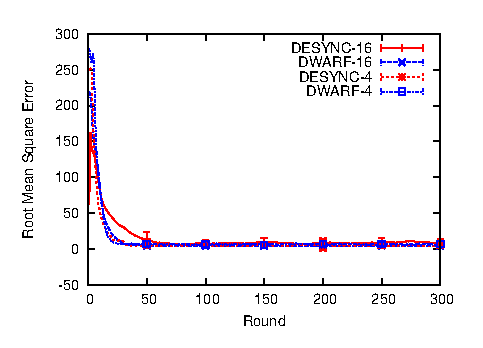
\includegraphics[width=2.0in]{figure/compare-rmse-4-16nodes_sd}%
	\label{fig:rmse-sparse}}
	\hfil
	\subfloat[Dense]{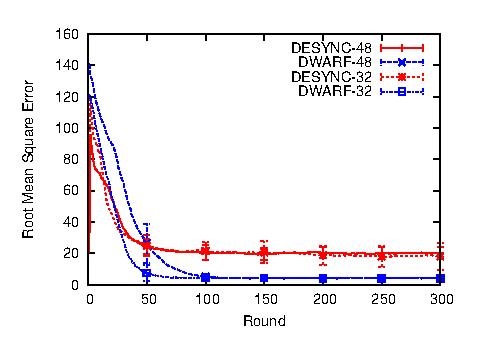
\includegraphics[width=2.0in]{figure/compare-rmse-32-48nodes_sd}%
	\label{fig:rmse-dense}}
	\hfil
	\subfloat[Extremely Dense]{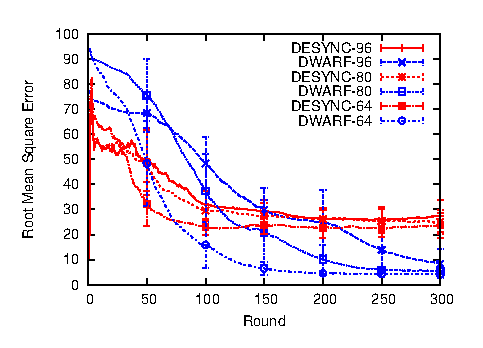
\includegraphics[width=2.0in]{figure/compare-rmse-64-80-96nodes_sd}%
	\label{fig:rmse-extreme}}
}
\caption{Convergence time and absolute root mean square error}
\label{fig:rmse-convergence}
\lofcont
\end{figure*}

\begin{figure*}[!t]
\centerline{
	\subfloat[Sparse]{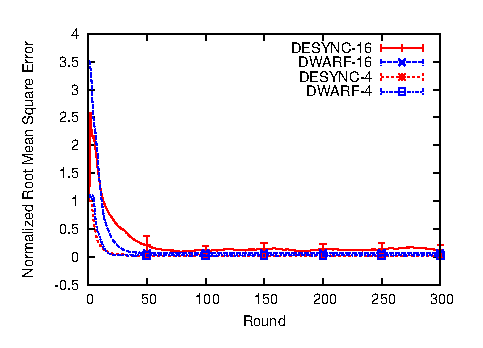
\includegraphics[width=2.0in]{figure/compare-nrmse-4-16nodes_sd}%
	\label{fig:nrmse-sparse}}
	\hfil
	\subfloat[Dense]{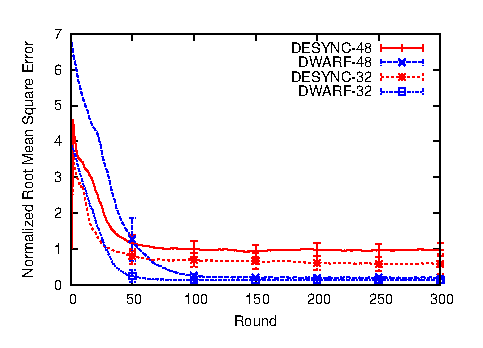
\includegraphics[width=2.0in]{figure/compare-nrmse-32-48nodes_sd}%
	\label{fig:nrmse-dense}}
	\hfil
	\subfloat[Extremely Dense]{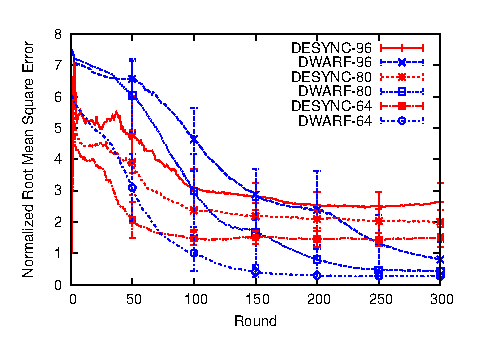
\includegraphics[width=2.0in]{figure/compare-nrmse-64-80-96nodes_sd}%
	\label{fig:nrmse-extreme}}
}
\caption{Convergence time and root mean square error normalized by expected phase difference}
\label{fig:nrmse-convergence}
\lofcont
\end{figure*}

\subsection{Correlation of Packet Loss and Desynchronization Error }
In this section, we investigate the correlation of packet loss and desynchronization error. 
We only include the results of DWARF in networks of 16, 48, and 80 nodes for 300 time periods (Figure \ref{fig:error-loss}). 
However, in networks of 4, 32, 64, and 96 nodes, the results are similar (not shown).

At the beginning, the network is far from the perfect desynchrony state and messages from different nodes are simultaneously fired. 
This results in lost packets and errors.
However, over time, nodes gradually adapt their time phases. 
Consequently, the number of lost packets and the error also gradually drop.


\begin{figure*}[!t]
\centerline{
	\subfloat[16 nodes]{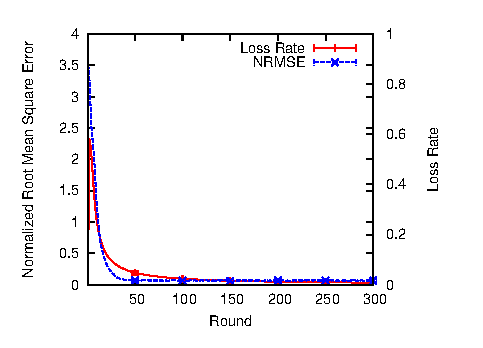
\includegraphics[width=2.2in]{figure/error-loss-16nodes_sd}%
	\label{fig:error-loss-16nodes}}
	\hfil
	\subfloat[48 nodes]{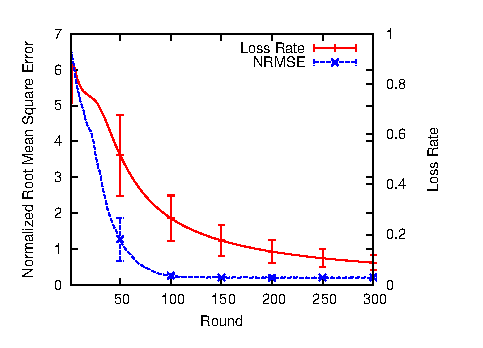
\includegraphics[width=2.2in]{figure/error-loss-48nodes_sd}%
	\label{fig:error-loss-48nodes}}
	\hfil
	\subfloat[80 nodes]{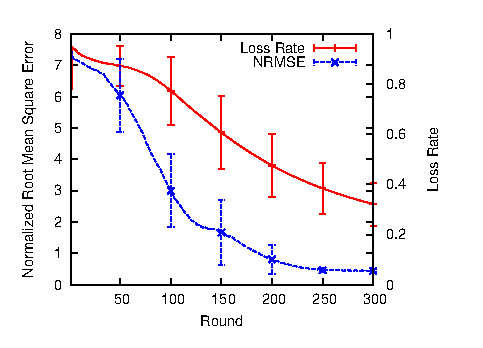
\includegraphics[width=2.2in]{figure/error-loss-80nodes_sd}%
	\label{fig:error-loss-80nodes}}
}
\caption{Correlation of packet loss and desynchronization error}
\label{fig:error-loss}
\lofcont
\end{figure*}
\section{Summary}
In this chapter, we present DWARF, a novel desynchronization algorithm that enables nodes in a system to perform tasks at different time. To the best of our knowledge, DWARF is the first desynchronization algorithm that is based on the concept of electromagnetic fields, a foundation of physics.
Our algorithm is completely distributed and localized with no reliance on a centralized node or a global notion of time. Due to low complexity in terms of computation, memory, and message overhead, DWARF is suitable for traditional wireless networks as well as resource-constraint wireless sensor networks. Our result indicates that DWARF can significantly outperform DESYNC by reducing 10 - 63\% of the desynchronization error. In addition, DWARF scales well with network size given that the normalized error is lower than 1 even in extremely dense networks.

The evaluation result of DWARF is promising. This result indicates that physicomimetics approach is viable for desynchronization. However, the evaluation has been performed on single-hop networks. Typically, wireless sensor networks are multi-hop networks. There are several issues to be concerned in extending DWARF to such networks. We cover such issues and present the multi-hop extension of DWARF in Chapter \ref{chap:multihop}.
Additionally, the evaluation does not show the mathematical evidence that the algorithm is stable and does not indicate why the algorithm converges. Therefore, we analyses the stability of the algorithm in the next chapter.



